\documentclass{beamer}
\begin{document}
\section{Message Passing}

\subsection{Introduction}
\begin{frame}
	\centering
	\large Unit-II\\
	\huge Message Passing
\end{frame}


\begin{frame}
	\frametitle{Introduction}
		Two basic methods for for information sharing as as follows
		\begin{enumerate}
		\item Shared Data Approach\\
		\begin{figure}
			\centering
			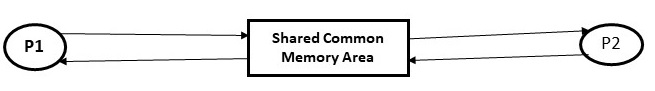
\includegraphics[width=10cm]{sharedDataApproach.jpg}\\
			\caption{Shared Data Approach}
		\end{figure}
		\item Message Passing Approach\\
		\begin{figure}
			\centering
			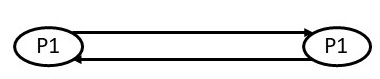
\includegraphics[width=10cm]{messagePassingApproach.jpg}
			\caption{Message Passing Approach}
		\end{figure}
		\end{enumerate}
\end{frame}


\begin{frame}
	\frametitle{Desirable Features of a good Message Passing System}
	\begin{enumerate}
		\item Simplicity
		\item Uniform Semantics
		\begin{itemize}
			\item Local Communication
			\item Remote Communication
		\end{itemize}
		\item Efficiency
		\item Reliability
		\item Correctness\\
			Issues related to correctness are
		\begin{itemize}
			\item Atomicity
			\item Ordered Delivery
			\item Survivability
		\end{itemize}
		\item Flexibility
		\item Security
		\item Portability
	\end{enumerate}
\end{frame}

\begin{frame}
	\frametitle{Issues in IPC by Message Passing}
	\justify{A message is a block of information formatted by a sending process in such a manner that it is meaningful to the receiving process.\\
	In the designing of an IPC protocol for message-passing system, the following important issues need to be considered.}
	\begin{figure}
		\centering
		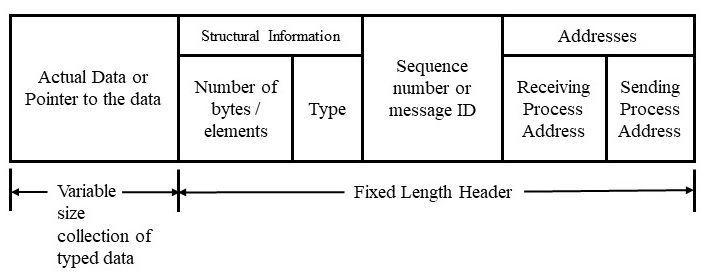
\includegraphics[width=10cm]{messageStructure.jpg}
		\caption{A Typical Message Structure}
	\end{figure}	
\end{frame}
\end{document}